\chapter{Evaluating the methods}
There are evidently a large variety of different methods available for solving the task at hand. Based on the work done in the previous chapter, this section of the paper will discuss possible solutions to the problem. 

\section{Available data}
One important aspect that should be considered is the amount of data available for the different methods. A key criterion for the success is that there exist satellite constellations that can provide frequently updated image data over the requested area. New images should be available on a weekly basis, and the resolution of the images has to be approximately one meter or less for the results to be accurate enough.

\subsection*{Multispectral images}
There are many different satellite constellations that provide frequently updated multispectral imagery of the requested area, such as the Sentinel-2 \citep{ESA}, SkySat \citep{Planet2017}, and WorldView \citep{DigitalGlobe2017} satellite constellations. All three constellations have a sub week revisit time over any point on earth. However, the ground sampling distance (GSD) varies with a factor of more than ten.

While both SkySat and WorldView provide a submeter accuracy on their images, the Sentinel-1 constellation has an expected GSD of 10x10 meters, which will not be sufficient for shadow measurements. Furthermore, it has to be taken into consideration that while data provided from the Sentinel constellations are free of charge, data from both SkySat and WorldView comes at a certain cost. Data provided by the Sentinel-2 constellation might, however, be accurate enough to locate the oil tanks. 

A general issue with multispectral images is that they are sensitive to cloudy weather and daylight. This can pose as an issue if the system is expected to continuously provide data without deviations.

\subsection*{Radar images}
Another type of images that are not affected by clouds or the time of day is radar images. In terms of radar-based methods, there are also a lot of satellite constellations that can be of interest. For example, while Sentinel-2 provide multispectral images, the Sentinel-1 constellation provides radar-images with resolutions down to 5x5 meters \citep{ESA}.

Other constellations, such as the TerraSAR-X can provide even higher resolutions as low as 1 meter, and the revisit time of the TerraSAR-X constellation has a revisit time of 11 days \citep{AirBus2017}. 

\section{Amount of data required for analysis}
An essential difference between the different methods presented in the previous sections is the amount of data needed to provide an accurate analysis. For example, simple image segmentation can be done in a single image using Simple Linear Iterative Clustering \citep{Achanta2012} as seen in \autoref{fig:superpixelsegmentation}. Furthermore, by knowing the approximate size of the oil tanks, a general Hough Transform \citep{Ballard1981} can be used to detect their circular shapes as seen in \autoref{fig:houghtransformcircles}. Image segmentation and shape detection using machine learning based methods require large amounts of training examples, which can be very hard to acquire. But as seen in \cite{Kaiser2017} and \cite{Kemker2017} it might be possible to automatically collect and label training data.

\begin{figure}[!h]
	\centering
	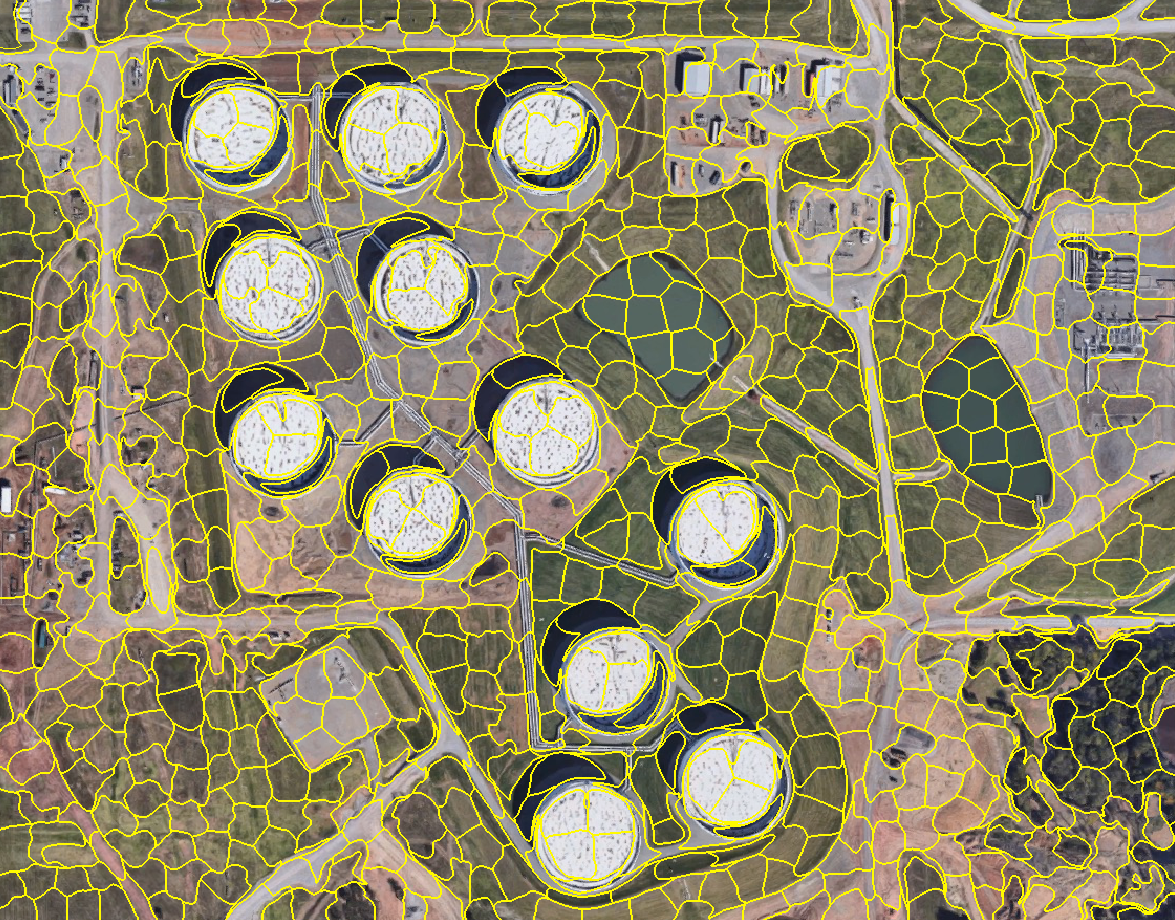
\includegraphics[scale=0.4]{fig/superpixel_segmentation.png}
	\caption{Simple implementation of SLIC superpixel segmentation on image taken from Google Earth}
	\label{fig:superpixelsegmentation}
\end{figure}

\begin{figure}[!h]
	\centering
	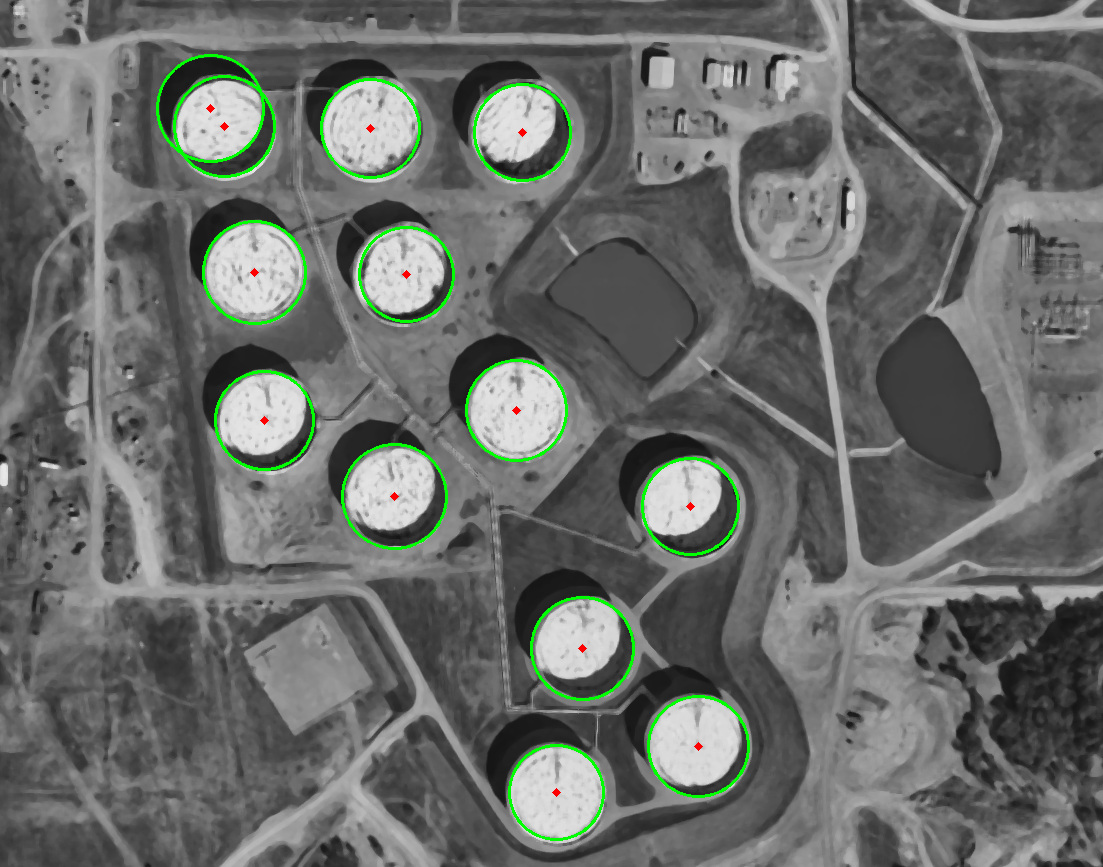
\includegraphics[scale=0.4]{fig/hough_transform_circles.png}
	\caption{Detecting circles of similar size in an image taken from Google Earth using a generalized hough transform}
	\label{fig:houghtransformcircles}
\end{figure}

Advanced methods in machine learning, such as Convolutional Neural Networks, have proven themselves as very efficient in image segmentation, but also in terms of classifying the different segments and even associating values with them if given the correct training data. This means that by acquiring the right training data, which in this setting would be the actual inventory of an oil tank at a specific time, and relate these values to aerial photographs of the same tanks, it would be possible to train a network into doing the actual inventory estimation directly.

When it comes to height estimation using radar images, \cite{Brunner2008} presented a method that only acquired a single radar image to estimate the height of buildings using the SAR principle. To generate an interferogram, two-phase images are required as explained in \cite{Liu2015}. Furthermore, height estimation using shadow measurement can also be done using single, multispectral images as shown by \cite{Comber2012} and \cite{Shao2011}.

\section{Choosing a method}
By taking the above comparison into consideration, it becomes clear that regarding pure circle detection, the generalized Hough transform stands out as the most efficient method. The fact that we have pre-knowledge about the shape of the objects we are trying to locate makes it much easier to use a standard approach. However, the generalized Hough transform will, isolated, not be able to estimate any heights, and would have to be combined with another method for height estimation. By looking at \autoref{fig:houghtransformcircles}, height estimation using shadow measurements might be the best approach. This is because the green circles limit the search area in terms of locating shadows since we are only interested in the shadow that is cast inside the tanks.

An important issue regarding the generalized Hough transform is the fact that if the tanks vary in size, it might not be able to find all of them, as seen in \autoref{fig:houghtransformdifference}.

\begin{figure}[!h]
	\centering
	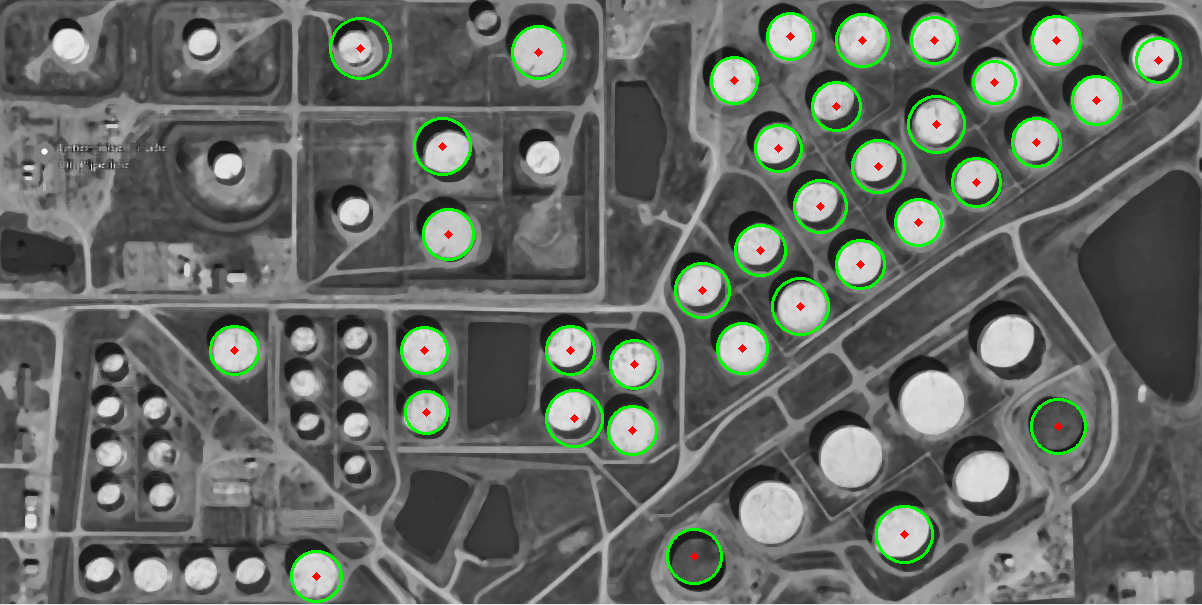
\includegraphics[scale=0.35]{fig/hough_transform_difference.png}
	\caption{Detecting circles of different size in an image taken from Google Earth using a generalized hough transform}
	\label{fig:houghtransformdifference}
\end{figure}

Looking at \autoref{fig:superpixelsegmentation} it seems like the SLIC algorithm has potential when it comes to image segmentation as well, but an issue is that it is hard to extract the correct edges without any prior knowledge. And the same issue regarding height estimation arises since the algorithm will have to be combined with another method.

As previously stated, it has been shown that convolutional neural networks outperform the state-of-the-art methods for image segmentation in terms of accuracy, if they are provided with enough good training examples. There are several ways to acquire training data, such as automatically extract training examples from OpenStreetMap as described by \cite{Kaiser2017}. 

Since 2012 convolutional networks have been the leading method for object recognition and image segmentation \citep{Krizhevsky2012}. Furthermore, very deep convolutional neural networks such as the ResNet \citep{Wu2017} have shown an incredible ability to create very complex functions for image analysis. The potential of these networks have yet not been fully explored, and there are still many applications that have not been discovered. One of them being building height extraction from aerial imagery.

By comparing the three presented methods for height estimation, it is clear that \cite{Brunner2008} presented the best results in terms of accuracy. However, both the relatively slow renewal time and the fact that the data can be quite challenging to acquire is something that has to be taken into account since the estimations should be done automatically at a sub-week frequency. Sentinel-1 provide this data automatically at a renewal time of 6 days, but with a less accurate resolution of 5x5 meters.

Even if \cite{Liu2015} did not achieve very high accuracy in their paper, there are still some aspects of interferometry that can be explored. The TanDEM-X mission is a mission is a public-private partnership between the German Aerospace Center and Airbus Defence and Space. The mission uses the TerraSAR-X and the TanDEM-X satellite to generate a high precision DEM, covering the whole planet. However, this DEM would have a renewal time of 11 days, which is, unfortunately, a too long period. Furthermore, as mentioned in \autoref{section:insar} interferograms can also be used to measure height differences over time. The problem with this is that the height difference between in a certain point cannot be more than 2.5 cm between two measurements, which would not be the case in terms of the height difference of the tank roof.

After comparing the different methods, it has become clear that there are many ways to attack the presented problem. Below two different methods are presented as potential approaches to solving the problem:

\begin{itemize}
    \item Direct estimation of the tanks inventory from shadow measurements in multispectral images, using a modified ResNet.
    \item Using a generalized Hough transform for tank detection, thus limiting the shadow search space, and then applying a modified ResNet for estimating a single tanks inventory in multispectral images.
\end{itemize}

\section{Implementation}
For the these methods to be tested, some aspects of implementation have to be considered. The main aspects are, what technology is needed to build the convolutional neural network and how can the data be acquired in order to train them.

\subsection*{Libraries for deep learning}
As a result of the vast development within the field of machine learning and especially neural networks, a lot of useful tools have been developed to aid the researchers in making it easier to implement new architectures. Two of these tools are Tensorflow and Keras.

\paragraph{Tensorflow} Tensorflow is an open source software library used for dataflow programming, and it is very much used for machine learning applications such as neural networks. Tensorflow was developed by the Google Brain team for internal use at Google but was later released under the Apache 2.0 open source license\footnote{Link: https://www.apache.org/licenses/LICENSE-2.0} in 2015.

\paragraph{Keras} Keras is an open source neural network library written in Python designed to enable fast experimentation with deep neural networks. The library runs on top of Tensorflow and contains numerous implementations of commonly used neural network building blocks.

By using these libraries in further research, it will be possible to test many different implementations of different networks, modify them and compare them with each other.

\subsection*{Gathering Data}
For a neural network to generalize beyond its training examples, it has to be provided with a substantial amount of labeled data. For example, the GoogleNet was trained on 1.2 million images when winning the ILSVRC 2014 challenge \citep{Szegedy2014}.  However, the amount of data required for training varies based on the task at hand. \cite{Wu2017} did an analysis based on the CIFAR-10 dataset, which consists of 50.000 training and 10.000 test images divided into 10different classes. By training their ResNet-110existthey achieved an accuracy of 6.43\%.

Of course, 50.000 training examples are still a lot of data, but it is substantially less than 1.2 million training examples.  Fortunately, it turns out that CNN's are good at transferring learning.  Meaning that once a network has been trained with an extensive database, it has adapted well enough to the structure of image data in general so that it can be adapted for a new task with relatively little training \citep{Marmanis2016}. 

There are several ways to attack the presented problem in terms of gathering enough data. Firstly, historical (as detailed as possible) of the inventory at Cushing has to be provided. There are many sources for this data, such as the U.Ss Energy information Administration which provides weekly, historical data back to 2004 of the total inventory.

Furthermore, this data has to be linked to time-stamped, high-resolution satellite images over the area.  This might become a problem for the earlier parts of the inventory data, but satellite data providers such as Digital Globe and Planet Labs large achieves which reach back many years.

Another approach is to train the network on something other than oil tanks, and then seeing how the network performs when trying to estimate the height difference between the tank walls and the roof. For example, it would be much simpler to train the network on trying to determine the height of buildings. This is because there exist large amounts of detailed building height models that can be combined with time-stamped, satellite images over areas that the height models represent. By combining these data sets, a significant amount of labeled training data can be generated.